\documentclass[10pt]{article}
\usepackage[a4paper,margin=18mm]{geometry}
\usepackage{amsmath,amssymb,booktabs,array,enumitem}
\usepackage[T1]{fontenc}\usepackage{lmodern}
\usepackage{tikz}\usetikzlibrary{shapes.gates.logic.US,positioning,arrows.meta,patterns,calc}
\usepackage[hidelinks]{hyperref}
\setlength{\parindent}{0pt}\setlength{\parskip}{4pt}
\setlength{\emergencystretch}{2em}
\newcommand{\VDD}{V_{DD}}
\newcommand{\mos}[4]{\begin{scope}[shift={(#1,#2)}]
\draw (0,.24)--(0,-.24);\draw (0,.20)--(.25,.20)--(.25,.5);
\draw (0,-.20)--(.25,-.20)--(.25,-.5);\draw (-.16,.23)--(-.16,-.23);
\ifnum#4=1\draw (-.26,0) circle (.06);\draw (-.75,0)--(-.32,0);\else\draw (-.75,0)--(-.16,0);\fi
\node[anchor=east,font=\scriptsize] at (-.76,0) {$#3$};\end{scope}}
\newcommand{\ground}[2]{\draw (#1,#2)--(#1,{#2-.12});\draw ({#1-.17},{#2-.12})--({#1+.17},{#2-.12});\draw ({#1-.11},{#2-.20})--({#1+.11},{#2-.20});}
\newcommand{\rail}[3]{\draw (#1,#2)--(#1,{#2+.14});\node[above,font=\scriptsize] at (#1,{#2+.14}) {$#3$};}

\newcommand{\hmos}[4]{\begin{scope}[shift={(#1,#2)}]
\draw(-.24,0)--(.24,0);\draw(-.2,0)--(-.2,-.25)--(-.5,-.25);\draw(.2,0)--(.2,-.25)--(.5,-.25);
\draw(-.23,.16)--(.23,.16);
\ifnum#4=1\draw(0,.26)circle(.06);\draw(0,.32)--(0,.75);\else\draw(0,.16)--(0,.75);\fi
\node[below,font=\scriptsize]at(0,-.32){#3};\end{scope}}
\newcommand{\gnd}[2]{\ground{#1}{#2}}\begin{document}
\begin{center}{\large\bfseries EE3032 Introduction to VLSI Design -- Final}\end{center}
\textbf{Archive attribution: 2021. Partial source.} The supplied three-page PDF assembles photographed fragments with overlap. Missing wording is marked and skipped. Typed Q7(d)--(f) is kept in a separate, unverified supplement, not silently restored as original text.

\textbf{1. (15 points)} Fig. 1 shows a domino logic circuit realizing the Boolean function $Y=AB+C$. Complete the following questions.
\begin{center}\begin{tikzpicture}[x=.85cm,y=.85cm,font=\scriptsize]
\node[and gate US,draw,logic gate inputs=nn,minimum width=.8cm] (a)at(1,1){ };
\node[or gate US,draw,logic gate inputs=nn,minimum width=.8cm] (b)at(3,1){ };
\draw(a.input 1)--++(-.8,0)node[left]{$A$};\draw(a.input 2)--++(-.8,0)node[left]{$B$};\draw(a.output)--(b.input 1);\draw(b.input 2)--++(-.5,0)--++(0,-.7)--(-.2,-.1)node[left]{$C$};\draw(b.output)--++(.6,0)node[right]{$Y$};
\draw(1,1.4)--(1,1.85)node[above]{$\phi$};\draw(3,1.4)--(3,1.85)node[above]{$\phi$};\node at(2,-.55){(a)};
\begin{scope}[shift={(5.5,.3)}]\draw(0,0)node[left]{$\phi$}--(.3,0)--(.6,.6)--(1.7,.6)--(2,0)--(2.8,0)--(3.1,.6)--(4.2,.6)--(4.5,0)--(4.9,0);\node at(2.5,-.85){(b)};\end{scope}
\end{tikzpicture}\\Figure 1: (a) A domino logic circuit (b) clock waveform.\end{center}
\begin{enumerate}[label=(\alph*),leftmargin=7mm]
\item Draw the transistor-level schematic diagram of the domino logic circuit. (5 points)
\item Assume that the output rise time/fall time of the AND and OR gates are 3 ns/2 ns and 2.5 ns/2 ns, respectively. Calculate the minimum clock period of $\phi$ if the duty cycle of $\phi$ is 50\%. (5 points)
\item Assume that each transistor has the following characteristics: $C_d=0.1$ fF; $C_g=1$ fF; $I_{Lp}=1$ nA (PMOS leakage current); $I_{Ln}=2$ nA (NMOS leakage current). Also, the supply voltage is 1.8 V and the threshold voltage of logic 1 is 1.3 V. Could the circuit be operated correctly at the minimum clock period? Why? (5 points)
\end{enumerate}
\textbf{2. (10 points)} Figure 2 shows a Schmitt trigger circuit. If you apply an input signal as shown in the left figure to the Schmitt trigger circuit, the circuit outputs the signal as shown in the right figure. Assume that $\mu_n=2\mu_p$; the turn-on equivalent resistance of N1 transistor is $R$; the simple RC delay model is used to estimate the delay and $t_r=t_f=2RC$. Complete the following questions.
\begin{enumerate}[label=(\alph*),leftmargin=7mm]
\item Let $V_{tn}=|V_{tp}|=0.4$ V, $V_{DD}=2.0$ V, $V_T^+=1.4$ V, and $V_T^-=0.6$ V. If the size of N1 is $100\mathrm{nm}/40\mathrm{nm}$, determine the sizes of the transistors N2, N3, P1, P2, and P3. (5 points)
\item Fig. 2(b) shows a Schmitt trigger with controllable hysteresis by controlling $V_{hc}$. If you want to increase $V_T^+$, how do you adjust $V_{hc}$? (5 points)
\end{enumerate}
\begin{center}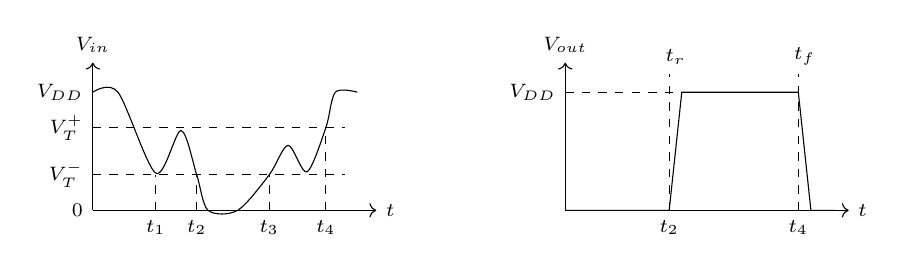
\begin{tikzpicture}[x=.8cm,y=.75cm,font=\scriptsize]
\draw[->](0,0)--(4.5,0)node[right]{$t$};\draw[->](0,0)--(0,2.5)node[above]{$V_{in}$};\node[left]at(0,2){$V_{DD}$};\node[left]at(0,1.4){$V_T^+$};\node[left]at(0,.6){$V_T^-$};\node[left]at(0,0){0};
\draw[dashed](0,1.4)--(4,1.4);\draw[dashed](0,.6)--(4,.6);\draw plot[smooth]coordinates{(0,2)(.4,2)(1,.63)(1.4,1.35)(1.65,.6)(1.83,0)(2.3,0)(2.8,.6)(3.1,1.1)(3.4,.65)(3.7,1.4)(3.85,2)(4.2,2)};
\foreach\x/\y/\t in {1/.6/1,1.65/.6/2,2.8/.6/3,3.7/1.4/4}{\draw[dashed](\x,0)--(\x,\y);\node[below]at(\x,0){$t_\t$};}
\begin{scope}[xshift=6cm]\draw[->](0,0)--(4.5,0)node[right]{$t$};\draw[->](0,0)--(0,2.5)node[above]{$V_{out}$};\draw(0,0)--(1.65,0)--(1.85,2)--(3.7,2)--(3.9,0)--(4.3,0);\draw[dashed](0,2)--(3.7,2);\draw[dashed](1.65,0)--(1.65,2.3);\draw[dashed](3.7,0)--(3.7,2.3);\node[above]at(1.75,2.3){$t_r$};\node[above]at(3.8,2.3){$t_f$};\node[left]at(0,2){$V_{DD}$};\node[below]at(1.65,0){$t_2$};\node[below]at(3.7,0){$t_4$};\end{scope}\end{tikzpicture}\\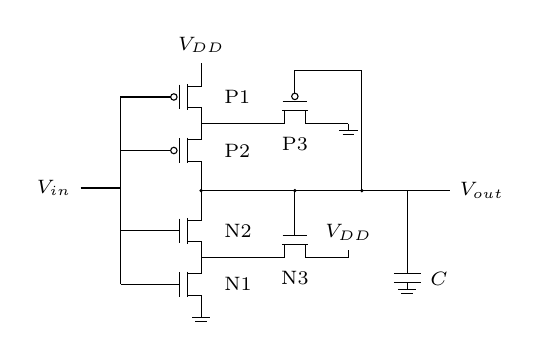
\begin{tikzpicture}[scale=0.68,font=\scriptsize]
\mos{1}{5}{}{1}\mos{1}{4}{}{1}\mos{1}{2.5}{}{0}\mos{1}{1.5}{}{0}
\rail{1.25}{5.5}{V_{DD}}\ground{1.25}{1}\draw(1.25,3)--(1.25,3.5);\draw(1.25,3.25)--(5.9,3.25)node[right]{$V_{out}$};\fill(1.25,3.25)circle(1pt);
\draw(-.25,1.5)--(-.25,5)--(.25,5);\draw(-.25,4)--(.25,4);\draw(-.25,2.5)--(.25,2.5);\draw(-.25,1.5)--(.25,1.5);\draw(-1,3.3)--(-.25,3.3)node[pos=0,left]{$V_{in}$};
\node[right]at(1.5,5){P1};\node[right]at(1.5,4){P2};\node[right]at(1.5,2.5){N2};\node[right]at(1.5,1.5){N1};
\hmos{3}{4.75}{P3}{1}\draw(1.25,4.5)--(2.5,4.5);\hmos{3}{2.25}{N3}{0}\draw(1.25,2)--(2.5,2);
\draw(3,3)--(3,3.25);\fill(3,3.25)circle(1pt);\draw(3,5.5)--(4.25,5.5)--(4.25,3.25);\fill(4.25,3.25)circle(1pt);
\draw(3.5,4.5)--(4,4.5);\ground{4}{4.5}\draw(3.5,2)--(4,2);\rail{4}{2}{V_{DD}}
\draw(5.1,3.25)--(5.1,1.7);\draw(4.85,1.7)--(5.35,1.7);\draw(4.85,1.53)--(5.35,1.53);\ground{5.1}{1.53}\node[right]at(5.35,1.6){$C$};
\end{tikzpicture}\quad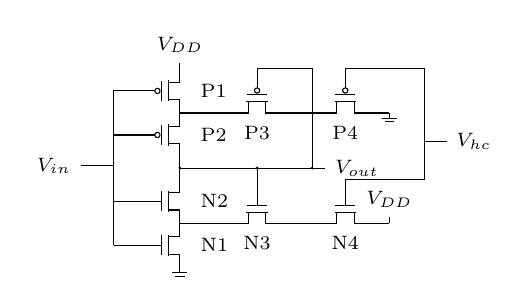
\begin{tikzpicture}[scale=0.56,font=\scriptsize]
\mos{1}{5}{}{1}\mos{1}{4}{}{1}\mos{1}{2.5}{}{0}\mos{1}{1.5}{}{0}
\rail{1.25}{5.5}{V_{DD}}\ground{1.25}{1}\draw(1.25,3)--(1.25,3.5);\draw(1.25,3.25)--(4.55,3.25)node[right]{$V_{out}$};\fill(1.25,3.25)circle(1pt);
\draw(-.25,1.5)--(-.25,5)--(.25,5);\draw(-.25,4)--(.25,4);\draw(-.25,2.5)--(.25,2.5);\draw(-.25,1.5)--(.25,1.5);\draw(-1,3.3)--(-.25,3.3)node[pos=0,left]{$V_{in}$};
\node[right]at(1.5,5){P1};\node[right]at(1.5,4){P2};\node[right]at(1.5,2.5){N2};\node[right]at(1.5,1.5){N1};
\hmos{3}{4.75}{P3}{1}\draw(1.25,4.5)--(2.5,4.5);\hmos{3}{2.25}{N3}{0}\draw(1.25,2)--(2.5,2);
\draw(3,3)--(3,3.25);\fill(3,3.25)circle(1pt);\draw(3,5.5)--(4.25,5.5)--(4.25,3.25);\fill(4.25,3.25)circle(1pt);
\hmos{5}{4.75}{P4}{1}\draw(3.5,4.5)--(4.5,4.5);\draw(5.5,4.5)--(6,4.5);\ground{6}{4.5}
\hmos{5}{2.25}{N4}{0}\draw(3.5,2)--(4.5,2);\draw(5.5,2)--(6,2);\rail{6}{2}{V_{DD}}
\draw(5,3)--(6.8,3)--(6.8,5.5)--(5,5.5);\draw(6.8,3.85)--(7.3,3.85)node[right]{$V_{hc}$};
\end{tikzpicture}\\Figure 2: (a) CMOS Schmitt trigger (b) trigger with controllable hysteresis.\end{center}
\newpage
\textbf{3. (10 points)} Draw the transistor-level schematic diagram of the Boolean function $f=\overline{AB(C+D)}$ using each of the following logic design styles: (1) Dynamic logic (5 points) (2) Differential split-level logic (5 points).

\textbf{4. (10 points)} Draw the transistor-level schematic diagram of the symbolic layout shown in Figure 3.
\begin{center}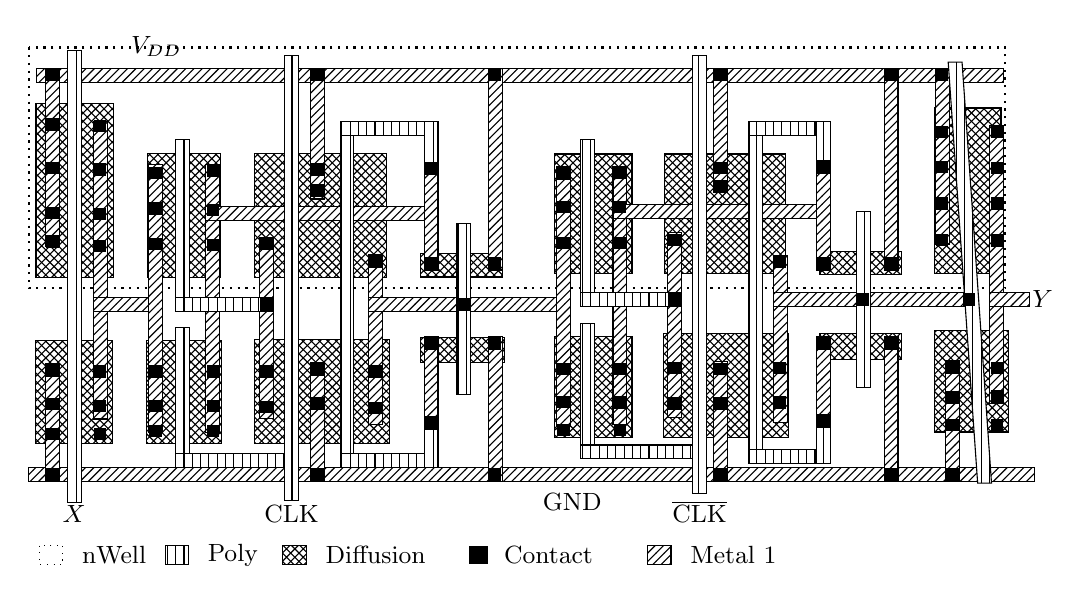
\begin{tikzpicture}[x=.011cm,y=-.011cm,font=\small]
\tikzset{lm/.style={preaction={fill=white},pattern=north east lines,pattern color=black},ld/.style={preaction={fill=white},pattern=crosshatch,pattern color=black},lp/.style={preaction={fill=white},pattern=vertical lines,pattern color=black}}
\draw[dotted,thick](273,108)rectangle(1400,386);
\draw[ld](281,173)rectangle(370,374);
\draw[ld](410,230)rectangle(494,374);
\draw[ld](533,230)rectangle(686,374);
\draw[ld](725,346)rectangle(820,373);
\draw[ld](880,231)rectangle(969,369);
\draw[ld](1006,231)rectangle(1146,369);
\draw[ld](1186,344)rectangle(1280,370);
\draw[ld](1318,178)rectangle(1395,369);
\draw[ld](280,446)rectangle(369,565);
\draw[ld](409,446)rectangle(495,565);
\draw[ld](533,445)rectangle(689,565);
\draw[ld](725,443)rectangle(822,472);
\draw[ld](880,442)rectangle(969,558);
\draw[ld](1005,438)rectangle(1150,558);
\draw[ld](1186,438)rectangle(1280,468);
\draw[ld](1318,435)rectangle(1404,552);
\draw[lm](282.0,132.0)rectangle(1398.0,148.0);
\draw[lm](272.0,593.0)rectangle(1434.0,609.0);
\draw[lm](292.0,132.0)rectangle(308.0,338.0);
\draw[lm](292.0,473.0)rectangle(308.0,609.0);
\draw[lm](347.0,194.0)rectangle(363.0,537.0);
\draw[lm](347.0,397.0)rectangle(427.0,413.0);
\draw[lm](411.0,243.0)rectangle(427.0,553.0);
\draw[lm](477.0,243.0)rectangle(493.0,553.0);
\draw[lm](477.0,292.0)rectangle(745.0,308.0);
\draw[lm](729.0,239.0)rectangle(745.0,365.0);
\draw[lm](539.0,327.0)rectangle(555.0,536.0);
\draw[lm](598.0,132.0)rectangle(614.0,283.0);
\draw[lm](598.0,472.0)rectangle(614.0,609.0);
\draw[lm](665.0,347.0)rectangle(681.0,543.0);
\draw[lm](665.0,397.0)rectangle(898.0,413.0);
\draw[lm](803.0,132.0)rectangle(819.0,365.0);
\draw[lm](803.0,442.0)rectangle(819.0,609.0);
\draw[lm](729.0,442.0)rectangle(745.0,550.0);
\draw[lm](882.0,246.0)rectangle(898.0,546.0);
\draw[lm](947.0,245.0)rectangle(963.0,543.0);
\draw[lm](947.0,289.0)rectangle(1198.0,305.0);
\draw[lm](1182.0,237.0)rectangle(1198.0,365.0);
\draw[lm](1010.0,322.0)rectangle(1026.0,535.0);
\draw[lm](1063.0,132.0)rectangle(1079.0,276.0);
\draw[lm](1063.0,471.0)rectangle(1079.0,609.0);
\draw[lm](1132.0,348.0)rectangle(1148.0,541.0);
\draw[lm](1132.0,391.0)rectangle(1366.0,407.0);
\draw[lm](1260.0,132.0)rectangle(1276.0,365.0);
\draw[lm](1260.0,442.0)rectangle(1276.0,609.0);
\draw[lm](1182.0,442.0)rectangle(1198.0,548.0);
\draw[lm](1319.0,132.0)rectangle(1335.0,335.0);
\draw[lm](1331.0,470.0)rectangle(1347.0,609.0);
\draw[lm](1382.0,198.0)rectangle(1398.0,519.0);
\draw[lm](1382.0,391.0)rectangle(1428.0,407.0);
\draw[lp](317.0,112.0)rectangle(333.0,633.0);
\draw[lp](442.0,214.0)rectangle(458.0,413.0);
\draw[lp](442.0,397.0)rectangle(555.0,413.0);
\draw[lp](442.0,431.0)rectangle(458.0,593.0);
\draw[lp](442.0,577.0)rectangle(584.0,593.0);
\draw[lp](568.0,117.0)rectangle(584.0,631.0);
\draw[lp](632.0,194.0)rectangle(648.0,593.0);
\draw[lp](632.0,194.0)rectangle(745.0,210.0);
\draw[lp](729.0,194.0)rectangle(745.0,255.0);
\draw[lp](632.0,577.0)rectangle(745.0,593.0);
\draw[lp](729.0,534.0)rectangle(745.0,593.0);
\draw[lp](767.0,311.0)rectangle(783.0,509.0);
\draw[lp](910.0,214.0)rectangle(926.0,407.0);
\draw[lp](910.0,391.0)rectangle(1026.0,407.0);
\draw[lp](910.0,427.0)rectangle(926.0,583.0);
\draw[lp](910.0,567.0)rectangle(1055.0,583.0);
\draw[lp](1039.0,117.0)rectangle(1055.0,623.0);
\draw[lp](1104.0,194.0)rectangle(1120.0,588.0);
\draw[lp](1104.0,194.0)rectangle(1198.0,210.0);
\draw[lp](1182.0,194.0)rectangle(1198.0,253.0);
\draw[lp](1104.0,572.0)rectangle(1198.0,588.0);
\draw[lp](1182.0,532.0)rectangle(1198.0,588.0);
\draw[lp](1228.0,297.0)rectangle(1244.0,501.0);
\draw[lp](1334,125)--(1350,125)--(1384,611)--(1368,611)--cycle;
\draw[fill=black](293.5,133.5)rectangle(306.5,146.5);
\draw[fill=black](293.5,594.5)rectangle(306.5,607.5);
\draw[fill=black](540.5,398.5)rectangle(553.5,411.5);
\draw[fill=black](730.5,240.5)rectangle(743.5,253.5);
\draw[fill=black](730.5,535.5)rectangle(743.5,548.5);
\draw[fill=black](768.5,398.5)rectangle(781.5,411.5);
\draw[fill=black](1011.5,392.5)rectangle(1024.5,405.5);
\draw[fill=black](1183.5,238.5)rectangle(1196.5,251.5);
\draw[fill=black](1183.5,533.5)rectangle(1196.5,546.5);
\draw[fill=black](1229.5,392.5)rectangle(1242.5,405.5);
\draw[fill=black](1351.5,392.5)rectangle(1364.5,405.5);
\draw[fill=black](599.5,133.5)rectangle(612.5,146.5);
\draw[fill=black](599.5,594.5)rectangle(612.5,607.5);
\draw[fill=black](804.5,133.5)rectangle(817.5,146.5);
\draw[fill=black](804.5,594.5)rectangle(817.5,607.5);
\draw[fill=black](1064.5,133.5)rectangle(1077.5,146.5);
\draw[fill=black](1064.5,594.5)rectangle(1077.5,607.5);
\draw[fill=black](1261.5,133.5)rectangle(1274.5,146.5);
\draw[fill=black](1261.5,594.5)rectangle(1274.5,607.5);
\draw[fill=black](1320.5,133.5)rectangle(1333.5,146.5);
\draw[fill=black](1332.5,594.5)rectangle(1345.5,607.5);
\draw[fill=black](293.5,190.5)rectangle(306.5,203.5);
\draw[fill=black](293.5,240.5)rectangle(306.5,253.5);
\draw[fill=black](293.5,292.5)rectangle(306.5,305.5);
\draw[fill=black](293.5,325.5)rectangle(306.5,338.5);
\draw[fill=black](348.5,192.5)rectangle(361.5,205.5);
\draw[fill=black](348.5,242.5)rectangle(361.5,255.5);
\draw[fill=black](348.5,293.5)rectangle(361.5,306.5);
\draw[fill=black](348.5,330.5)rectangle(361.5,343.5);
\draw[fill=black](412.5,246.5)rectangle(425.5,259.5);
\draw[fill=black](412.5,287.5)rectangle(425.5,300.5);
\draw[fill=black](412.5,328.5)rectangle(425.5,341.5);
\draw[fill=black](478.5,244.5)rectangle(491.5,257.5);
\draw[fill=black](478.5,289.5)rectangle(491.5,302.5);
\draw[fill=black](478.5,329.5)rectangle(491.5,342.5);
\draw[fill=black](540.5,328.5)rectangle(553.5,341.5);
\draw[fill=black](599.5,242.5)rectangle(612.5,255.5);
\draw[fill=black](599.5,266.5)rectangle(612.5,279.5);
\draw[fill=black](666.5,348.5)rectangle(679.5,361.5);
\draw[fill=black](730.5,350.5)rectangle(743.5,363.5);
\draw[fill=black](804.5,350.5)rectangle(817.5,363.5);
\draw[fill=black](883.5,247.5)rectangle(896.5,260.5);
\draw[fill=black](883.5,285.5)rectangle(896.5,298.5);
\draw[fill=black](883.5,327.5)rectangle(896.5,340.5);
\draw[fill=black](948.5,246.5)rectangle(961.5,259.5);
\draw[fill=black](948.5,285.5)rectangle(961.5,298.5);
\draw[fill=black](948.5,327.5)rectangle(961.5,340.5);
\draw[fill=black](1011.5,323.5)rectangle(1024.5,336.5);
\draw[fill=black](1064.5,240.5)rectangle(1077.5,253.5);
\draw[fill=black](1064.5,261.5)rectangle(1077.5,274.5);
\draw[fill=black](1133.5,349.5)rectangle(1146.5,362.5);
\draw[fill=black](1183.5,350.5)rectangle(1196.5,363.5);
\draw[fill=black](1261.5,350.5)rectangle(1274.5,363.5);
\draw[fill=black](1320.5,199.5)rectangle(1333.5,212.5);
\draw[fill=black](1320.5,239.5)rectangle(1333.5,252.5);
\draw[fill=black](1320.5,281.5)rectangle(1333.5,294.5);
\draw[fill=black](1320.5,323.5)rectangle(1333.5,336.5);
\draw[fill=black](1383.5,199.5)rectangle(1396.5,212.5);
\draw[fill=black](1383.5,240.5)rectangle(1396.5,253.5);
\draw[fill=black](1383.5,281.5)rectangle(1396.5,294.5);
\draw[fill=black](1383.5,324.5)rectangle(1396.5,337.5);
\draw[fill=black](293.5,474.5)rectangle(306.5,487.5);
\draw[fill=black](293.5,513.5)rectangle(306.5,526.5);
\draw[fill=black](293.5,547.5)rectangle(306.5,560.5);
\draw[fill=black](348.5,475.5)rectangle(361.5,488.5);
\draw[fill=black](348.5,515.5)rectangle(361.5,528.5);
\draw[fill=black](348.5,547.5)rectangle(361.5,560.5);
\draw[fill=black](412.5,475.5)rectangle(425.5,488.5);
\draw[fill=black](412.5,515.5)rectangle(425.5,528.5);
\draw[fill=black](412.5,544.5)rectangle(425.5,557.5);
\draw[fill=black](478.5,475.5)rectangle(491.5,488.5);
\draw[fill=black](478.5,515.5)rectangle(491.5,528.5);
\draw[fill=black](478.5,544.5)rectangle(491.5,557.5);
\draw[fill=black](540.5,475.5)rectangle(553.5,488.5);
\draw[fill=black](540.5,516.5)rectangle(553.5,529.5);
\draw[fill=black](599.5,473.5)rectangle(612.5,486.5);
\draw[fill=black](599.5,512.5)rectangle(612.5,525.5);
\draw[fill=black](666.5,475.5)rectangle(679.5,488.5);
\draw[fill=black](666.5,517.5)rectangle(679.5,530.5);
\draw[fill=black](730.5,443.5)rectangle(743.5,456.5);
\draw[fill=black](804.5,443.5)rectangle(817.5,456.5);
\draw[fill=black](883.5,472.5)rectangle(896.5,485.5);
\draw[fill=black](883.5,510.5)rectangle(896.5,523.5);
\draw[fill=black](883.5,543.5)rectangle(896.5,556.5);
\draw[fill=black](948.5,472.5)rectangle(961.5,485.5);
\draw[fill=black](948.5,511.5)rectangle(961.5,524.5);
\draw[fill=black](948.5,543.5)rectangle(961.5,556.5);
\draw[fill=black](1011.5,471.5)rectangle(1024.5,484.5);
\draw[fill=black](1011.5,512.5)rectangle(1024.5,525.5);
\draw[fill=black](1064.5,472.5)rectangle(1077.5,485.5);
\draw[fill=black](1064.5,512.5)rectangle(1077.5,525.5);
\draw[fill=black](1133.5,471.5)rectangle(1146.5,484.5);
\draw[fill=black](1133.5,511.5)rectangle(1146.5,524.5);
\draw[fill=black](1183.5,443.5)rectangle(1196.5,456.5);
\draw[fill=black](1261.5,443.5)rectangle(1274.5,456.5);
\draw[fill=black](1332.5,471.5)rectangle(1345.5,484.5);
\draw[fill=black](1332.5,505.5)rectangle(1345.5,518.5);
\draw[fill=black](1332.5,537.5)rectangle(1345.5,550.5);
\draw[fill=black](1383.5,471.5)rectangle(1396.5,484.5);
\draw[fill=black](1383.5,504.5)rectangle(1396.5,517.5);
\draw[fill=black](1383.5,537.5)rectangle(1396.5,550.5);
\node[above]at(420,130){$V_{DD}$};\node[below]at(900,612){GND};
\node[below]at(325,626){$X$};\node[below]at(576,626){CLK};\node[below]at(1047,620){$\overline{\mathrm{CLK}}$};\node[right]at(1420,399){$Y$};
\draw[dotted](285,683)rectangle(312,705);\node[right]at(323,694){nWell};
\draw[lp](430,683)rectangle(457,705);
\node[right]at(468,694){Poly};
\draw[ld](566,683)rectangle(593,705);
\node[right]at(604,694){Diffusion};
\draw[fill=black](782.0,684.0)rectangle(802.0,704.0);
\node[right]at(810,694){Contact};
\draw[lm](987,683)rectangle(1014,705);
\node[right]at(1025,694){Metal 1};
\end{tikzpicture}\\Figure 3: Symbolic layout.\end{center}

\textbf{5. (20 points)} Fig. 4(a) shows a CMOS circuit driving a large capacitance $C_L=2.98$ pF. For the used process, the input capacitance $C_g$ of a minimum-size inverter (i.e., the size of NMOS and PMOS is $W_{min}/L_{min}$) is 1 fF. Assume that drain and wire parasitic capacitance can be neglected. Also, $e=2.7$, $e^4=55$, $e^6=403$, and $e^8=2980$. Complete the following questions:
\begin{enumerate}[label=(\alph*),leftmargin=7mm]
\item Design a super buffer as shown in Fig. 4(b) to drive the large capacitance such that the output load of NAND gate A is $C_g$ and the delay $T$ is minimized. (7 points)
\item Assume that we apply the input sequence $00\to01\to10\to11\to00$ to the circuit in terms of the operation frequency $f$ and the supply voltage $V_{dd}$.
\begin{enumerate}[label=\roman*.,leftmargin=6mm]
\item Calculate the switching activity of nodes $u,v,w,o$. (5 points)
\item Calculate the dynamic power consumed by the super buffer. (5 points)
\item If the two NAND gates have the same delay, does this circuit have spurious transitions (glitches)? Why? (3 points)
\end{enumerate}\end{enumerate}
\begin{center}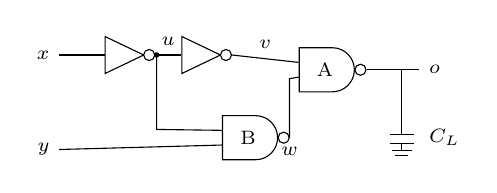
\begin{tikzpicture}[x=.75cm,y=.75cm,font=\scriptsize]
\node[not gate US,draw,minimum width=.55cm](i1)at(1,2){};\node[not gate US,draw,minimum width=.55cm](i2)at(2.3,2){};\node[nand gate US,draw,logic gate inputs=nn,minimum width=.7cm](a)at(4.5,1.75){A};\node[nand gate US,draw,logic gate inputs=nn,minimum width=.7cm](b)at(3.2,.6){B};
\draw(i1.input)--(0,2)node[left]{$x$};\draw(i1.output)--(i2.input)node[midway,above]{$u$};\draw(i2.output)--(a.input 1)node[midway,above]{$v$};\draw(b.output)--(3.9,.6)--(3.9,1.6)--(a.input 2);\draw(1.65,2)--(1.65,.74)--(b.input 1);\fill(1.65,2)circle(1pt);\draw(0,.4)node[left]{$y$}--(b.input 2);
\draw(a.output)--(6.1,1.75)node[right]{$o$};
\node[below]at(3.9,.6){$w$};
\draw(5.8,1.75)--(5.8,.65);\draw(5.6,.65)--(6.0,.65);\draw(5.6,.5)--(6.0,.5);\ground{5.8}{.5}\node[right]at(6.1,.6){$C_L$};
\end{tikzpicture}\quad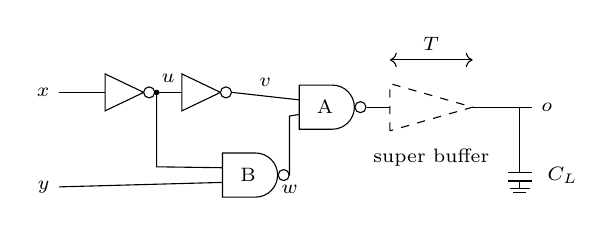
\begin{tikzpicture}[x=.75cm,y=.75cm,font=\scriptsize]
\node[not gate US,draw,minimum width=.55cm](i1)at(1,2){};\node[not gate US,draw,minimum width=.55cm](i2)at(2.3,2){};\node[nand gate US,draw,logic gate inputs=nn,minimum width=.7cm](a)at(4.5,1.75){A};\node[nand gate US,draw,logic gate inputs=nn,minimum width=.7cm](b)at(3.2,.6){B};
\draw(i1.input)--(0,2)node[left]{$x$};\draw(i1.output)--(i2.input)node[midway,above]{$u$};\draw(i2.output)--(a.input 1)node[midway,above]{$v$};\draw(b.output)--(3.9,.6)--(3.9,1.6)--(a.input 2);\draw(1.65,2)--(1.65,.74)--(b.input 1);\fill(1.65,2)circle(1pt);\draw(0,.4)node[left]{$y$}--(b.input 2);
\draw(a.output)--(5.6,1.75);\draw[dashed](5.6,1.35)--(5.6,2.15)--(7,1.75)--cycle;\node[below]at(6.3,1.2){super buffer};\draw(7,1.75)--(8,1.75)node[right]{$o$};\draw[<->](5.6,2.55)--(7,2.55)node[midway,above]{$T$};
\node[below]at(3.9,.6){$w$};
\draw(7.8,1.75)--(7.8,.65);\draw(7.6,.65)--(8.0,.65);\draw(7.6,.5)--(8.0,.5);\ground{7.8}{.5}\node[right]at(8.1,.6){$C_L$};
\end{tikzpicture}\\Figure 4: (a) NAND gate driving a large capacitance (b) inserted super buffer.\end{center}
\newpage
\textbf{6. (15 points; incomplete)} Figure 5 shows a sequential circuit. Assume that the clock-to-Q propagation delay ($t_{pcq}$), the clock-to-Q contamination delay ($t_{ccq}$), the setup time ($t_{setup}$), and the hold time ($t_{hold}$) of the [text continues beyond the photograph crop].

\textbf{Missing original text:} numerical timing assumptions, the remaining opening text, and Q6(a),(b) are cropped out. They cannot be answered and are skipped.

\textbf{Readable Q6(c):} Inserting registers into the circuit such that the modified circuit can be operated at 2 times of the original operation frequency. (5 points)

\textbf{Cannot answer Q6(c):} the original timing parameters and preceding conditions are unavailable. The diagram and readable wording are retained; no target clock, register count, or numerical redesign is inferred from student work.
\begin{center}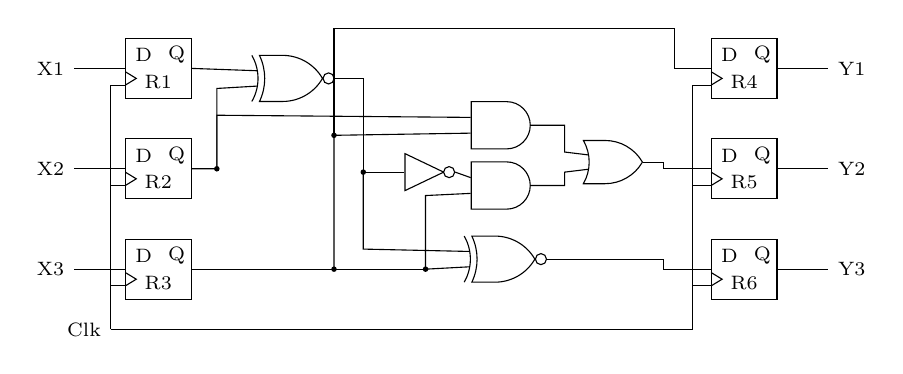
\begin{tikzpicture}[x=.93cm,y=.85cm,font=\scriptsize]
\foreach\r/\y in {1/4,2/2.5,3/1}{\draw(0,\y-.45)rectangle(.9,\y+.45);\node at(.25,\y+.2){D};\node at(.7,\y+.2){Q};\node at(.45,\y-.2){R\r};\draw(-.7,\y)--(0,\y);\node[left]at(-.7,\y){X\r};\draw(0,\y-.25)--(.15,\y-.15)--(0,\y-.05);}
\foreach\r/\y/\o in {4/4/Y1,5/2.5/Y2,6/1/Y3}{\draw(8,\y-.45)rectangle(8.9,\y+.45);\node at(8.25,\y+.2){D};\node at(8.7,\y+.2){Q};\node at(8.45,\y-.2){R\r};\draw(8.9,\y)--(9.6,\y)node[right]{\o};\draw(8,\y-.25)--(8.15,\y-.15)--(8,\y-.05);}
\draw(-.2,.1)node[left]{Clk}--(7.75,.1);\draw(-.2,.1)--(-.2,3.75);\foreach\y in {3.75,2.25,.75}{\draw(-.2,\y)--(0,\y);}\draw(7.75,.1)--(7.75,3.75);\foreach\y in {3.75,2.25,.75}{\draw(7.75,\y)--(8,\y);}
\node[xnor gate US,draw,logic gate inputs=nn,minimum width=.8cm](s)at(2.2,3.85){};\draw(.9,4)--(s.input 1);\draw(.9,2.5)--(1.25,2.5)--(1.25,3.7)--(s.input 2);
\node[and gate US,draw,logic gate inputs=nn,minimum width=.75cm](h)at(5.1,3.15){};\node[and gate US,draw,logic gate inputs=nn,minimum width=.75cm](l)at(5.1,2.25){};\node[or gate US,draw,logic gate inputs=nn,minimum width=.75cm](o)at(6.6,2.6){};\node[not gate US,draw,minimum width=.55cm](n)at(4,2.45){};\node[xnor gate US,draw,logic gate inputs=nn,minimum width=.8cm](p)at(5.1,1.15){};
\draw(s.output)--(3.25,3.85)--(3.25,2.45)--(n.input);\draw(3.25,2.45)--(3.25,1.3)--(p.input 1);\fill(3.25,2.45)circle(1pt);
\draw(n.output)--(l.input 1);\draw(1.25,2.5)--(1.25,3.3)--(h.input 1);\fill(1.25,2.5)circle(1pt);
\draw(.9,1)--(4.1,1);\draw(2.85,1)--(2.85,3)--(h.input 2);\draw(2.85,3)--(2.85,4.6)--(7.5,4.6)--(7.5,4)--(8,4);\fill(2.85,3)circle(1pt);\fill(2.85,1)circle(1pt);\draw(4.1,1)--(p.input 2);\draw(4.1,1)--(4.1,2.1)--(l.input 2);\fill(4.1,1)circle(1pt);
\draw(h.output)--(6,3.15)--(6,2.75)--(o.input 1);\draw(l.output)--(6,2.25)--(6,2.45)--(o.input 2);\draw(o.output)--(7.35,2.6)--(7.35,2.5)--(8,2.5);\draw(p.output)--(7.35,1.15)--(7.35,1)--(8,1);
\end{tikzpicture}\\Figure 5: A sequential circuit.\end{center}
\textbf{7. (25 points; original latter parts missing)} Answer the following questions.
\begin{enumerate}[label=(\alph*),leftmargin=7mm]
\item List two requirements for drawing the layout of a cell in the standard cell library. (4 points)
\item List two limitations of dynamic logic. (4 points)
\item What is the goal of the design rule? (3 points)
\end{enumerate}
Readable Q7(d) fragment: ``A pseudo-NMOS logic is'' [remainder cropped]. The original Q7(d)--(f) cannot be fully read and are skipped as original exam questions.

\textbf{Separate unverified typed supplement from the supplied PDF:}
\begin{enumerate}[label=(\alph*),start=4,leftmargin=7mm]
\item A pseudo-NMOS logic is ratioed-logic. Why?
\item What's the function of filler cell, tap cell, endcap cell, decap cell?
\item List two technology that can shorten manufactured time and hence shorten the time to market.
\end{enumerate}
The supplied typed note speculates that the last answer means gate-array and sea-of-gates physical design. This comment is secondary evidence, not original wording or an official answer. No missing point values are invented. Printed whole-question totals sum to 105; original labels are retained.
\end{document}
